\section{Design}

CLAS12 Trigger System is designed as 3-stage pipeline-style system with total latency up to 8us. Stage 1 receives information from various CLAS12 detecrors and performs data processing in according to the type of detector. Stage 2 performs timing and geometry coincidence between different subset of dectors in 6 groups in according to 6-sector CLAS12 detector structure, as well as coincidence with information from central detectors. Stage 3 forms final trigger decision.
CLAS12 Trigger diagram is shown on Fig.~\ref{fig:TriggerDiagram}.

\begin{figure}[hbt]
	\centering
	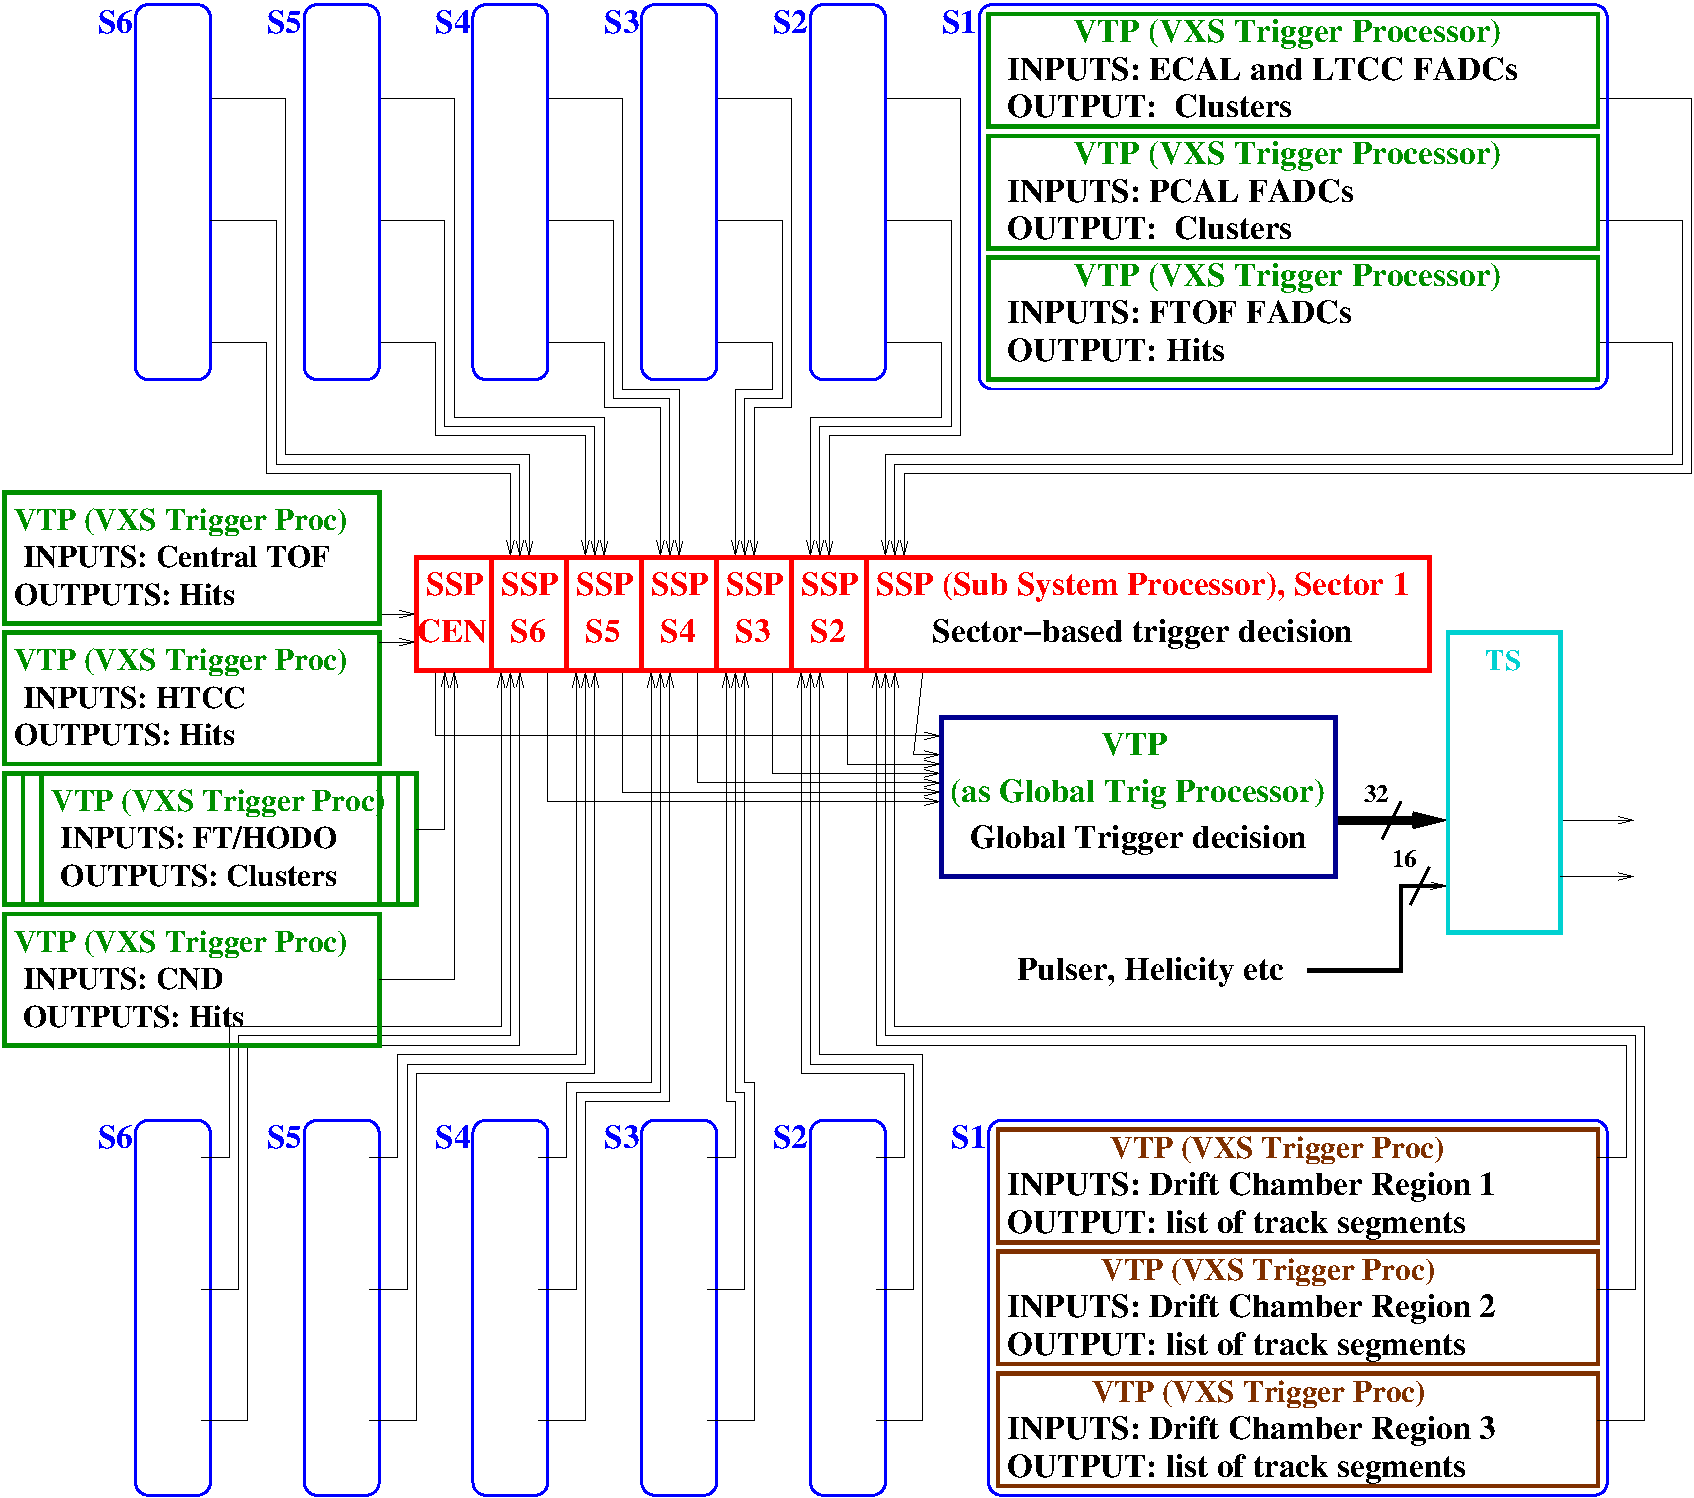
\includegraphics[width=1.0\columnwidth,keepaspectratio]{img/CLAS12_TRIGGER_1.pdf}
	\caption{CLAS12 Trigger System Diagram}
	\label{fig:TtiggerDiagram}
\end{figure}


\subsection{Stage 1} The most complex processing is performed for electromagnetic calorimeters (cluster finding) and drift chamber tracker (segment and road finding).

\subsubsection{Electromagnetic calorimeters} sergey

\subsubsection{Drift Chamber} sergey,ben

\subsubsection{High Threshold Cherenkov Counter} sergey

\subsubsection{Forward Time-Of-Flight Counter} sergey

\subsubsection{Central Time-Of-Flight Counter} sergey

\subsubsection{Neutron Detector} sergey

\subsubsection{Forward Calorimeter and Hodoscope} andrea,ben


\subsection{Stage 2} ben


\subsection{Stage 3} ben

